\section{基于投影与参数得分的分类}
\label{sec:classification-linear-score}

前面章节已经说明，分类器可以把特征加权相加成一个实值得分，再由得分的正负或大小决定类别。本节直接规定由输入得到投影、仿射得分或条件概率的参数关系，再分别从监督散度、错误修正、逐步间隔投影、最大间隔和条件似然中学习参数。这些方法共享同一个可计算的得分接口，训练依据却各自建立：Fisher准则比较投影后的类间分离与类内波动，感知机按错分样本修正参数，被动攻击算法在单条记录上作最小改动的间隔投影，SVM在批量目标中选择最大间隔，Logistic回归与Softmax回归则直接拟合条件概率。线性与核化是表示选择，不与概率输出组成互斥类别；同一个得分形式不意味着同一个学习目标。

\subsection{Fisher判别分析}
\label{sec:classification-fisher}

用花瓣长度与宽度区分两类鸢尾花时，只比较两类平均长度可能遗漏宽度提供的信息，把两项测量直接相加也未必合适：如果某项测量在同类花之间波动很大，它区分类别的作用可能不及另一项；两项测量相关时，还要考虑它们是否重复提供同一份信息。Fisher在1936年的鸢尾花分类研究中寻找一种线性组合，使两类均值的差异相对于类内波动尽可能大\scite{fisher1936}。这一准则不要求样本服从高斯分布；它与后面第\ref{sec:classification-gda}节的高斯生成模型可以给出相同的判别方向，但概率解释和适用条件有所不同。

\subsubsection{模型结构}
\label{sec:classification-fisher-structure}

二分类中，Fisher把输入投影到一个单位方向上，再按投影位置判类。设方向参数为$\bm{w}\in\mathbb{R}^{d}$（不预先归一化），投影得分为
\begin{equation}
  z(\bm{x})=\bm{w}^{\top}\bm{x},
\end{equation}
阈值规则为$\hat y(\bm{x})=+1$当$z(\bm{x})\geq t$，否则$-1$；平局按固定顺序处理。这里$\bm{w}$只负责把两类在一条轴上拉开，$t$负责在该轴上划界；方向本身不报告后验概率，也不假设输入服从某种类条件分布。需要预先说明的是，这个$\bm{w}$不是沿某条损失梯度逐步估计的权重，而是由两类散度矩阵的广义特征值问题从训练数据闭式解出的投影方向；散度矩阵本身也只是对训练样本的统计汇总。多类投影需要同时保留多个判别方向，本节先建立二分类的单方向投影与两类判断。

\subsubsection{参数学习}
\label{sec:classification-fisher-learning}

投影是否有效，要看投影后类中心分开多远、同类样本挤得多紧。令$n_c=\sum_i\mathbb{1}\{y_i=c\}$，各类均值与总样本均值为
\[
  \hat{\bm{\mu}}_c=\frac1{n_c}\sum_{i:y_i=c}\bm{x}_i,\qquad
  \hat{\bm{\mu}}=\sum_{c=1}^{C}\frac{n_c}{n}\hat{\bm{\mu}}_c.
\]
定义\term{类内散度矩阵}（within-class scatter matrix）与\term{类间散度矩阵}（between-class scatter matrix）：
\begin{equation}
  \begin{aligned}
    \bm{S}_{\mathrm{W}}
      &=\sum_{c=1}^{C}\sum_{i:y_i=c}
        (\bm{x}_i-\hat{\bm{\mu}}_c)
        (\bm{x}_i-\hat{\bm{\mu}}_c)^{\top},\\
    \bm{S}_{\mathrm{B}}
      &=\sum_{c=1}^{C}n_c
        (\hat{\bm{\mu}}_c-\hat{\bm{\mu}})
        (\hat{\bm{\mu}}_c-\hat{\bm{\mu}})^{\top}.
  \end{aligned}
  \label{eq:classification-fisher-scatter}
\end{equation}
$\bm{S}_{\mathrm{W}}$累加每个样本相对于本类中心的偏离，衡量类内波动；$\bm{S}_{\mathrm{B}}$衡量各类中心相对于总中心的分散程度。投影到方向$\bm{w}$后，两种散度分别变为$\bm{w}^{\top}\bm{S}_{\mathrm{B}}\bm{w}$和$\bm{w}^{\top}\bm{S}_{\mathrm{W}}\bm{w}$。\term{Fisher判别准则}（Fisher discriminant criterion）取两者之比；以下假设$\bm{S}_{\mathrm{W}}\succ0$，使每个非零方向的分母都为正：
\begin{equation}
  J(\bm{w})
    =\frac{\bm{w}^{\top}\bm{S}_{\mathrm{B}}\bm{w}}
          {\bm{w}^{\top}\bm{S}_{\mathrm{W}}\bm{w}},
  \qquad \bm{w}\ne\bm{0}.
  \label{eq:classification-fisher-criterion}
\end{equation}
分子鼓励类中心远离，分母抑制同类样本投影后过于分散。

图~\ref{fig:classification-lda-projection}固定同一组二维教学样本，只改变单位投影方向。两类中心分别为$(-1,0)^{\top}$与$(1,0)^{\top}$，每类都加上偏移$(-0.3,-1)^{\top}$、$(-0.1,1)^{\top}$、$(0.1,1)^{\top}$、$(0.3,-1)^{\top}$。由这些点算得$\bm{S}_{\mathrm{W}}=\operatorname{diag}(2/5,8)$与$\bm{S}_{\mathrm{B}}=\operatorname{diag}(8,0)$，最优方向由$\bm{S}_{\mathrm{W}}^{-1}(\hat{\bm\mu}_2-\hat{\bm\mu}_1)$归一化得到$\bm w^\ast=(1,0)^{\top}$。它使投影均值相差$2$，合并类内方差为$0.05$；比较方向$\bm w_{\mathrm B}=(3/5,4/5)^{\top}$的均值间距为$1.2$、类内方差为$0.658$，所以两者的$J$分别为$20$与$180/329$。这里方差按总样本量$8$归一化；右侧浅色条只是样本投影的最小至最大范围，不能把它当作Fisher准则中的平方偏差。

\begin{figure}[htbp]
  \centering
  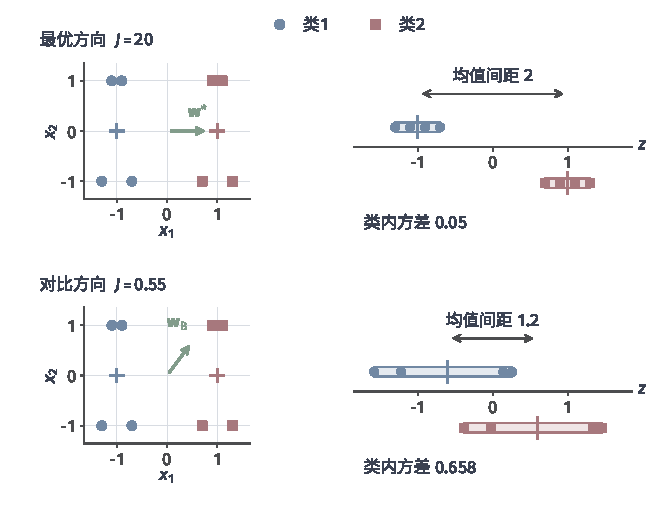
\includegraphics[width=112.000mm]{figures/04-classic-models/00-shared/matplotlib/classification-lda-target/figure.pdf}
  \caption{Fisher投影同时比较均值间距与类内散布。每类4个教学点，坐标无量纲；两行复用同一点集和相同投影数轴尺度。左侧绿色箭头为单位投影方向，十字为类均值；右侧短竖线为投影均值，浅色条为各类的样本投影范围，双向箭头标出均值间距。标注方差由$n^{-1}\bm w^{\top}\bm S_{\mathrm W}\bm w$计算，$J$仍按散度比计算。}
  \label{fig:classification-lda-projection}
\end{figure}

由于$J$不受$\bm{w}$的非零倍数缩放影响，可以约束$\bm{w}^{\top}\bm{S}_{\mathrm{W}}\bm{w}=1$。对$\bm{w}^{\top}\bm{S}_{\mathrm{B}}\bm{w}-\lambda(\bm{w}^{\top}\bm{S}_{\mathrm{W}}\bm{w}-1)$求导，得到\term{广义特征值问题}（generalized eigenvalue problem）：
\begin{equation}
  \bm{S}_{\mathrm{B}}\bm{w}
    =\lambda\bm{S}_{\mathrm{W}}\bm{w}.
  \label{eq:classification-fisher-eigenproblem}
\end{equation}
驻点还需比较大小。令$\bm{v}=\bm{S}_{\mathrm{W}}^{1/2}\bm{w}$，则
\[
  J(\bm{w})=\frac{\bm{v}^{\top}\bm{A}\bm{v}}{\bm{v}^{\top}\bm{v}},
  \qquad
  \bm{A}=\bm{S}_{\mathrm{W}}^{-1/2}
    \bm{S}_{\mathrm{B}}\bm{S}_{\mathrm{W}}^{-1/2}.
\]
把$\bm{v}$展开到对称半正定矩阵$\bm{A}$的正交特征向量上（半正定即任意方向上的二次型都非负），上式就是各特征值的加权平均，权重非负且总和为$1$。最大值因而是最大特征值；取对应特征向量，再乘$\bm{S}_{\mathrm{W}}^{-1/2}$，便得到最优Fisher方向。若最大特征值有重数，最优方向未必唯一。

二分类时，令$\bm{h}=\hat{\bm{\mu}}_1-\hat{\bm{\mu}}_2\ne\bm{0}$，由总均值的定义可得
\[
  \bm{S}_{\mathrm{B}}=\frac{n_1n_2}{n}\bm{h}\bm{h}^{\top},
  \qquad
  \bm{w}_{\mathrm{F}}\propto\bm{S}_{\mathrm{W}}^{-1}\bm{h}.
\]
即最优方向正比于$\bm{S}_{\mathrm{W}}^{-1}$作用在均值差上。生成式LDA的法向量则为$\bm{w}_{\mathrm{G}}=\hat{\bm{\Sigma}}^{-1}\bm{h}=n\bm{S}_{\mathrm{W}}^{-1}\bm{h}$，两者方向相同（见第\ref{sec:classification-gda}节）；但完整的生成式分类规则还要比较类先验与阈值，Fisher准则本身只给方向，不给类先验、后验概率或这一阈值。两类均值相同时，均值散度准则没有正特征值方向，而生成模型仍可按先验选择类别。因此Fisher投影可用于非高斯数据，贝叶斯最优性的证明则还需要正确指定的生成模型。散度奇异、某类样本不足时，正定参数域内的方向估计需要先降维或正则化，不能把奇异样本散度直接代入。

\subsubsection{支持非线性类别关系：核Fisher判别}
\label{sec:classification-kfd}

原坐标上的线性投影只能沿一个方向拉开类别。例如内外两圈样本在原坐标中的均值都可能接近原点，原坐标上的均值差便提供不了有用方向；增加距离平方等非线性特征后，两类在新坐标中才具有不同均值。Mika等提出的\term{核Fisher判别}（kernel Fisher discriminant, KFD）在特征空间中重新计算类均值与散度，再最大化投影后的类间与类内散度比\scite{mika1999kernel}。它改变的是输入表示，保留的仍是散度比较准则。

将投影方向写成$\bm{w}=\sum_{i=1}^n a_i\phi(\bm{x}_i)$，记$\bm a=(a_1,\ldots,a_n)^\top\in\mathbb R^n$，核矩阵$\bm K\in\mathbb R^{n\times n}$的元素为$\bm K_{i,j}=K(\bm x_i,\bm x_j)$。第$j$个训练样本的投影值为
\begin{equation}
  \begin{aligned}
    z_j&=\langle\bm w,\phi(\bm x_j)\rangle
        =\sum_{i=1}^n a_i K(\bm x_i,\bm x_j),\\
    \bm z&=\bm K\bm a,\qquad
      \bm z=(z_1,\ldots,z_n)^\top .
  \end{aligned}
  \label{eq:classification-kfd-projected-samples}
\end{equation}
第$c$类的投影均值为$\bar z_c=n_c^{-1}\sum_{j:y_j=c}z_j$，总投影均值为$\bar z=n^{-1}\sum_j z_j$。沿用前面的类间与类内散度定义，两个投影散度分别为
\begin{equation}
  \begin{aligned}
    s_{\mathrm B}(\bm a)
      &=\sum_{c=1}^C n_c(\bar z_c-\bar z)^2,\\
    s_{\mathrm W}(\bm a)
      &=\sum_{c=1}^C\sum_{j:y_j=c}(z_j-\bar z_c)^2 .
  \end{aligned}
  \label{eq:classification-kfd-projected-scatter}
\end{equation}
每个$z_j$以及上述均值都对$\bm a$线性，所以两个平方和都对$\bm a$二次；分母为正时，$s_{\mathrm B}(\bm a)/s_{\mathrm W}(\bm a)$就是原Fisher准则在特征空间中的写法。这样，只用核矩阵和类别标签便能计算候选方向的比值。若类内散度奇异，可以采用系数正则化，例如把分母改为$s_{\mathrm W}(\bm a)+\lambda_{\mathrm K}\lVert\bm a\rVert_2^2$，其中$\lambda_{\mathrm K}>0$；非零系数方向的分母因而严格为正。将两个散度分别展开为$\bm a^\top\bm B_K\bm a$和$\bm a^\top\bm W_K\bm a$，两个矩阵均为$n\times n$，就可按前面的Fisher推导求广义特征值问题$\bm B_K\bm a=\lambda(\bm W_K+\lambda_{\mathrm K}\bm I_n)\bm a$的最大特征值方向。训练完成后，新样本的投影得分为$z(\bm x)=\sum_i a_iK(\bm x_i,\bm x)$。二分类还需在这条轴上确定阈值，例如在相邻训练得分之间及两端外侧比较类别错误数，再用选定阈值给新输入判类；核参数和正则化强度通过训练集内部验证选择，这个阈值学习步骤不能由Fisher方向自动替代。

它与核SVM的区别仍在训练准则：KFD关注整体类统计量，SVM关注间隔及其违反程度。KFD的基本解通常没有支持向量式的稀疏性，预测可能需要访问全部训练样本；若要从投影得分得到后验概率，还需额外建立得分分布或校准模型。例如，内外两圈分别具有固定半径$1$与$2$时，径向特征$\phi(\bm x)=\|\bm x\|_2^2$把两类送到$1$与$4$，在二者之间设置阈值就能精确分开；若所选核仍只提供原坐标的线性组合，同中心两圈的均值差仍为零，Fisher准则便没有得到所需的径向信息。所选核是否保留径向信息，决定了这里的目标能否表达。
